\chapter{System Modeling} \label{cap:cap4}
\section{UML Diagrams}
\subsection{Use Case Diagrams}
\subsubsection{Event Management}
The use case in figure~\ref{fig:eventusecase} shows how a user can manage his agenda. After he logs into the platform he will see his calendar and being able to see schedule of his events. This event can be modified and so deleted or if the user is the event's owner he can invite other users.
 \begin{center}
 \begin{figure}[H]
    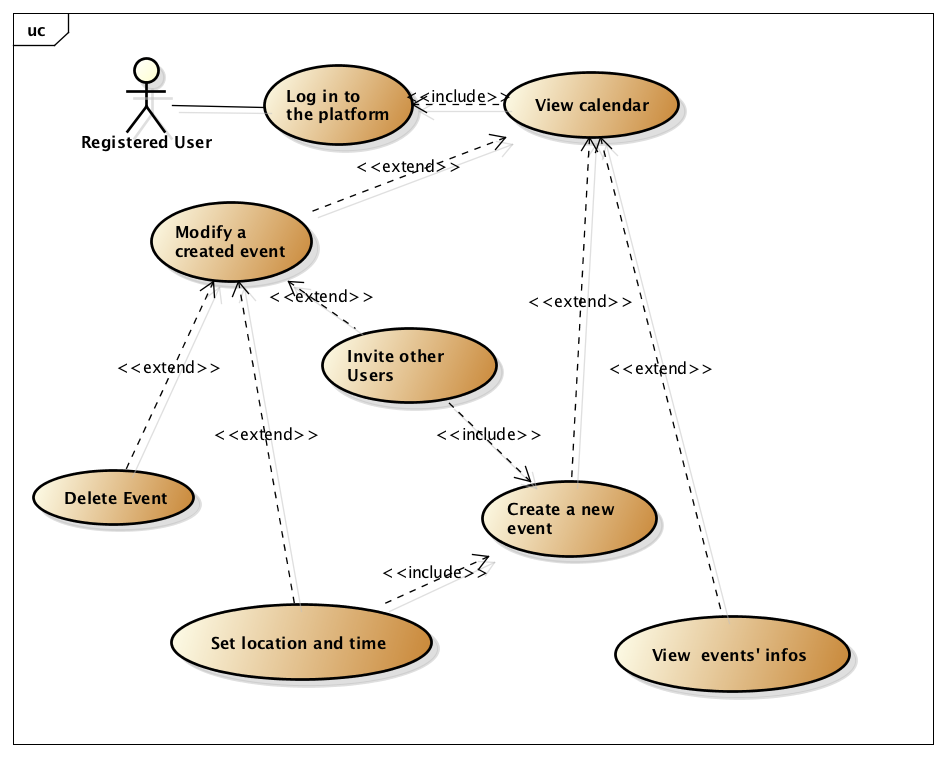
\includegraphics[width=1\textwidth]{../UMLDiagram/use_case/EventManagmentUseCase/EventManagment.png}
    \caption{Event Management Use Case}
     \label{fig:eventusecase}
     \end{figure}
   \end{center}  
The use case in the shows how a user can manage his agenda. After he logs into the platform he will see his calendar and being able to see schedule of his events.This events can be modified and so deleted or if he is the event's owner he can invite other users.This use case show how a user can manage his agenda. After he logs into the platform he will see his calendar and being able to see schedule of his events.This events can be modified and so deleted or if he is the event's owner he can invite other users.
\subsubsection{Invitation}
The use case in figure \ref{fig:invitusecase} explains what the user can do when he receive an invitation to an event from an other user. Once he get the notification he can either see the event's info and accept or decline the invite.\\\\\\
 \begin{center}
 \begin{figure}[H]
    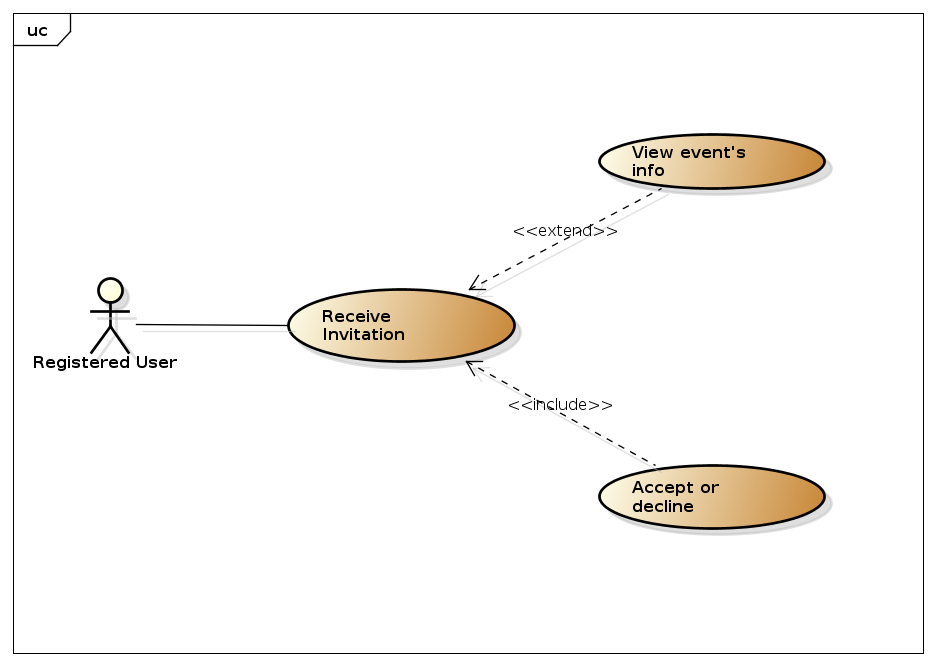
\includegraphics[width=1\textwidth]{../UMLDiagram/use_case/Invitation/Invitation.png}
    \caption{Invitation Use Case}
     \label{fig:invitusecase}
     \end{figure}
   \end{center}  
\subsubsection{View other profiles}
The use case in figure \ref{fig:otherprofileusecase} shows how an user can reach the profile of an other user and view his agenda. After he logs in to the platform he will be able to search an user and see his profile, but he will be authorized to see the other user's calendar only if it set as public by its owner.   
 \begin{center}
 \begin{figure}[H]
    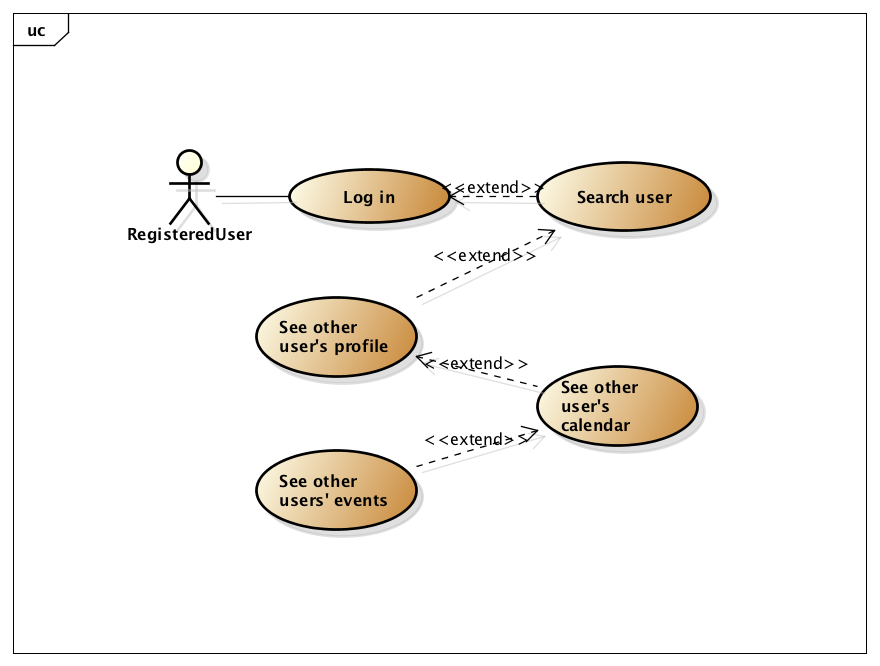
\includegraphics[width=1\textwidth]{../UMLDiagram/use_case/ViewOtherProfiles/UseCaseDiagram0.png}
    \caption{See Other User Profile Use Case}
     \label{fig:otherprofileusecase}
     \end{figure}
   \end{center}  
\subsubsection{Bad Weather}
The use case in figure \ref{fig:otherprofileusecase} explains how an user can behave when he get notified by the platform in case of bad weather condition. Whenever he receives a bad weather notifications the user can act in two different way. If he's the event's owner he can delete the event or modify the event's location while if he's an event's participant he can only manage his event's participation.
 \begin{center}
 \begin{figure}
    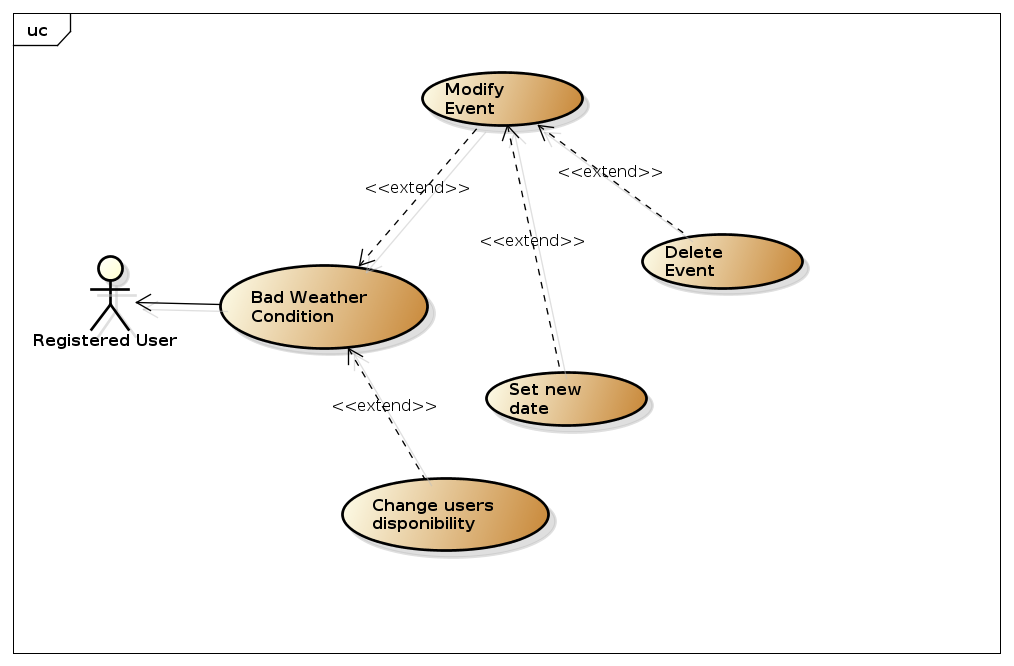
\includegraphics[width=1.1\textwidth]{../UMLDiagram/use_case/BadWeather/BadWeather.png}
    \caption{Bad Weather Use Case}
     \label{fig:badweatherusecase}
     \end{figure}
   \end{center}  
\subsection{Class Diagrams}
\begin{center}
 \begin{figure}
    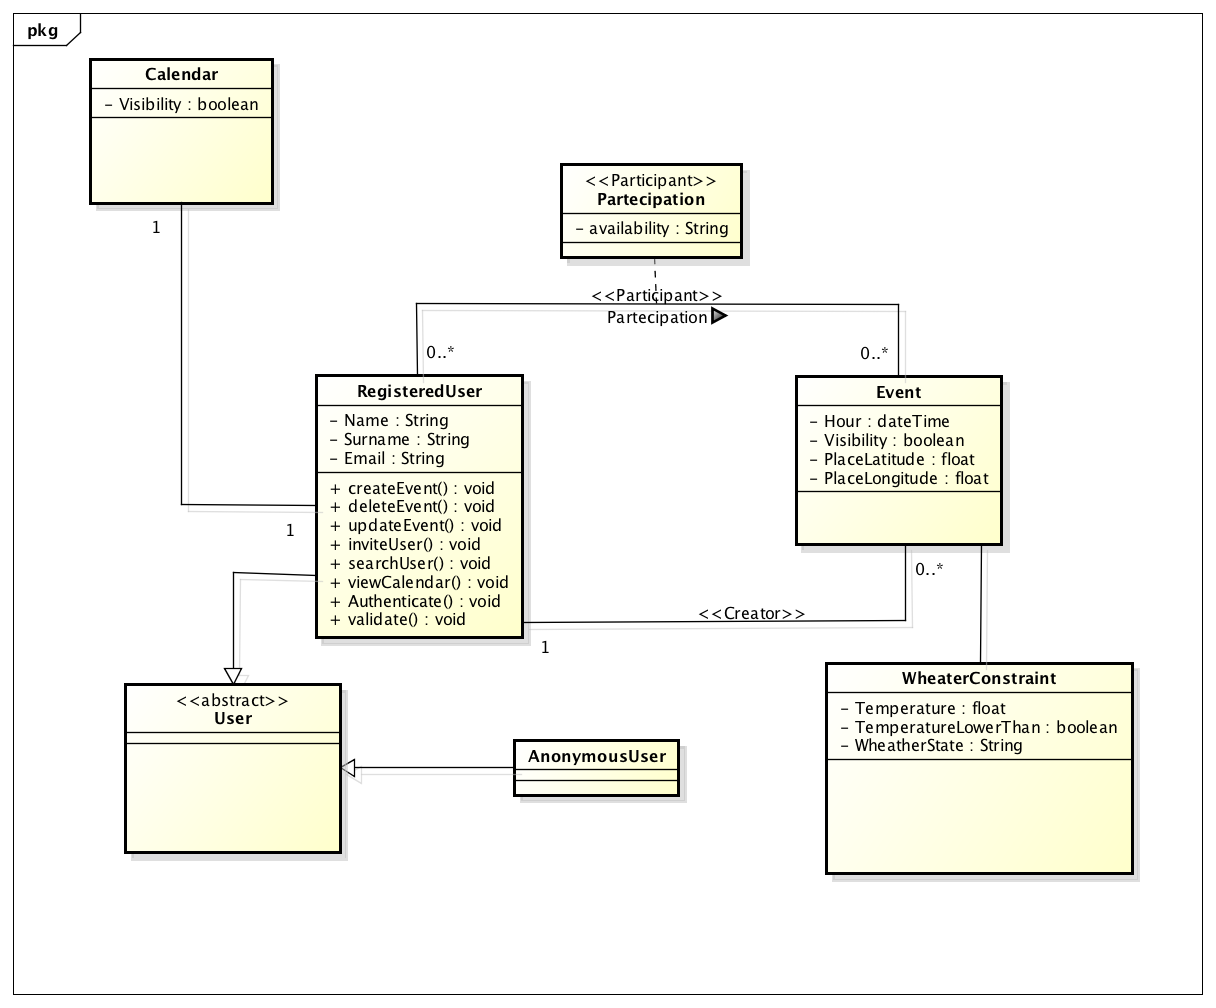
\includegraphics[width=1\textwidth]{../UMLDiagram/class/WeatherCalClassDiagram/ClassDiagram0.png}
    \caption{Class Diagram}
     \label{fig:classdiagram}
     \end{figure}
   \end{center}  
\subsection{State Diagrams}
\subsubsection{Invitation}
 \begin{center}
 \begin{figure}[H]
    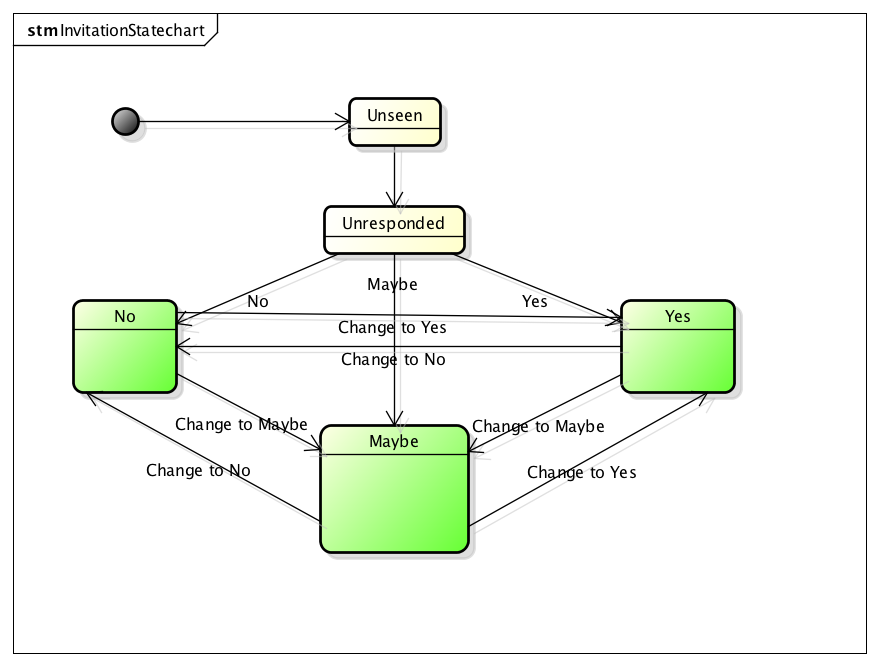
\includegraphics[width=1\textwidth ]{../UMLDiagram/InvitationStatechart/InvitationStatechart.png}
    \caption{Invitation State Diagram}
     \label{fig:invstatediagram}
     \end{figure}
   \end{center}  
 \subsection{Sequence Diagrams}
\subsubsection{User Registration}
\begin{center}
 \begin{figure}[H]
    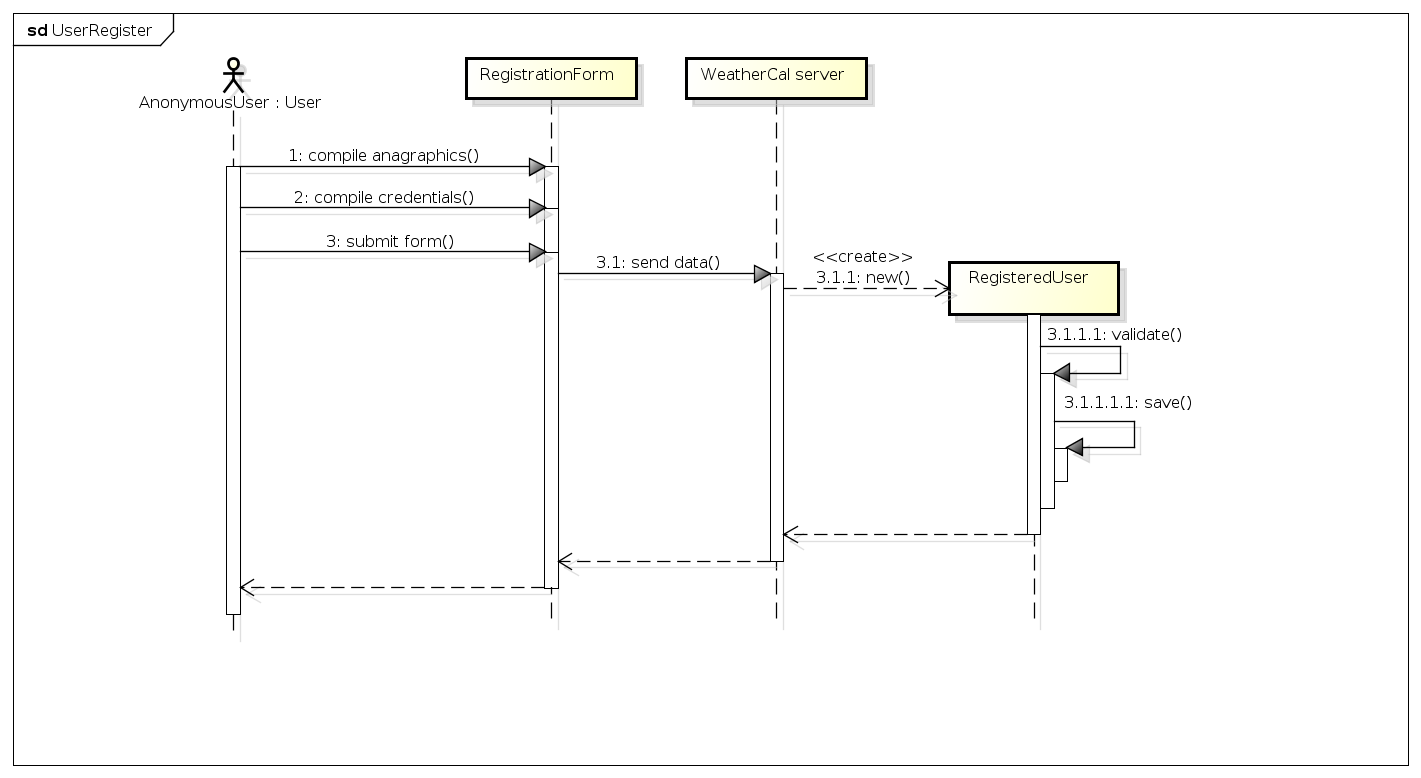
\includegraphics[width=1\textwidth]{../UMLDiagram/sequence/UserRegister/UserRegister.png}
    \caption{Sequence diagram of user registration}
     \label{fig:regseqdiag}
     \end{figure}
   \end{center}  

\subsubsection{Login}
\begin{center}
 \begin{figure}[H]
    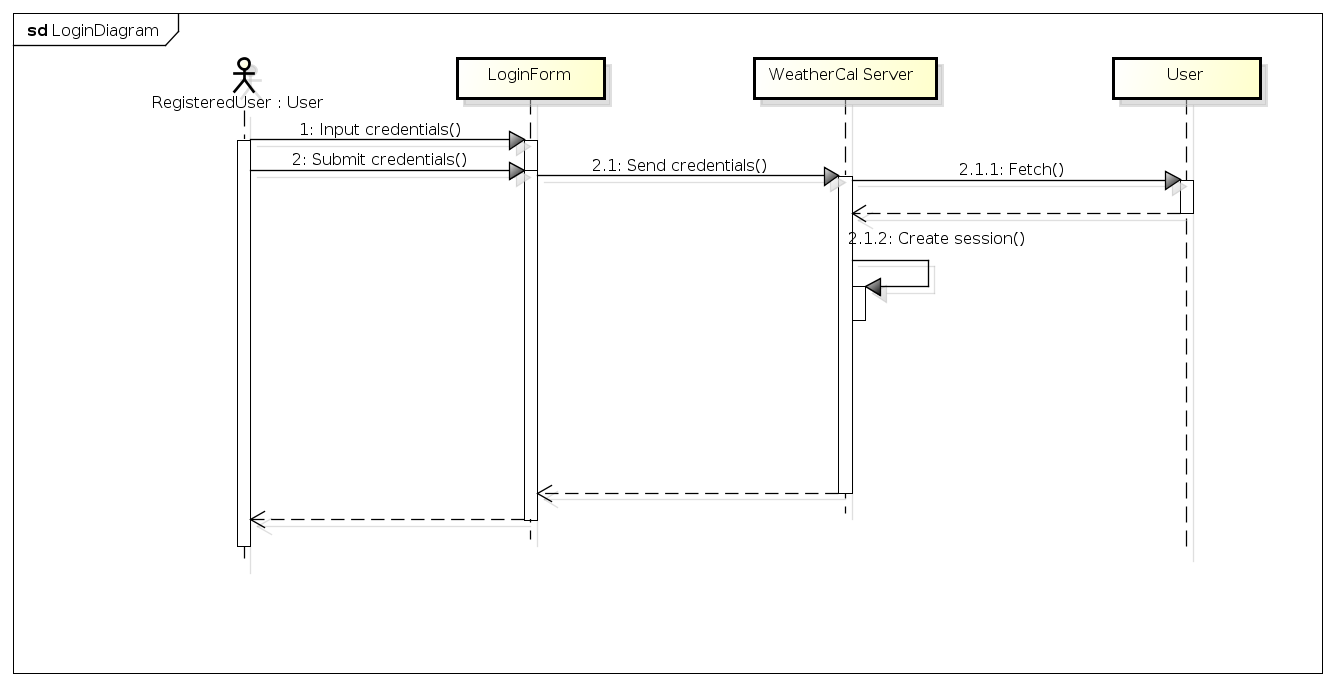
\includegraphics[width=1\textwidth]{../UMLDiagram/sequence/LoginDiagram/LoginDiagram.png}
    \caption{Login Sequence Diagram}
     \label{fig:logseqdiag}
     \end{figure}
   \end{center}  
\subsubsection{Event creation}
\begin{center}
 \begin{figure}[H]
    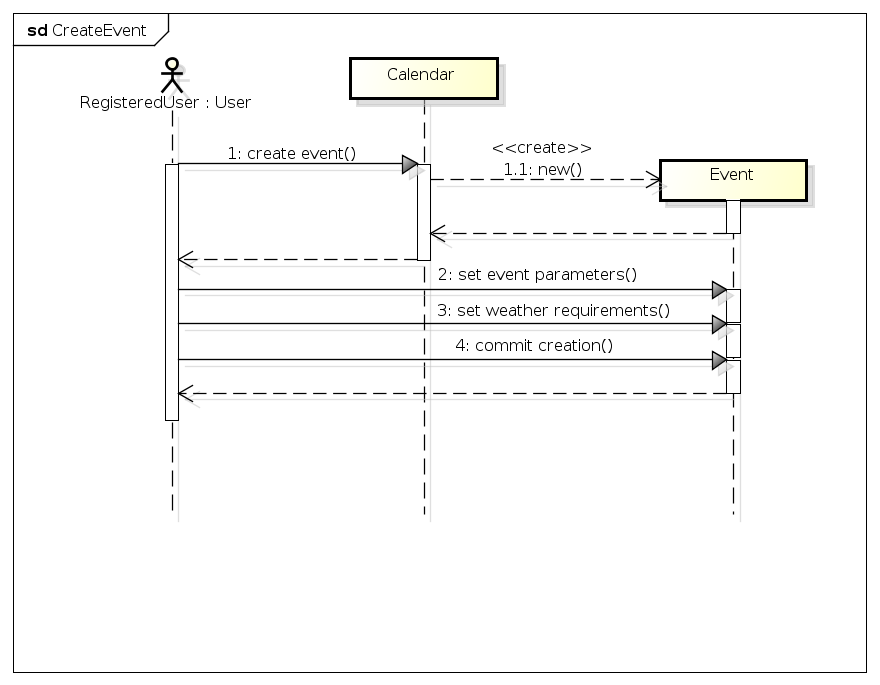
\includegraphics[width=1\textwidth]{../UMLDiagram/sequence/CreateEvent/CreateEvent.png}
    \caption{Create Event Sequence Diagram}
     \label{fig:createseqdiag}
     \end{figure}
   \end{center}  
\subsubsection{Event modification}
\begin{center}
 \begin{figure}[H]
    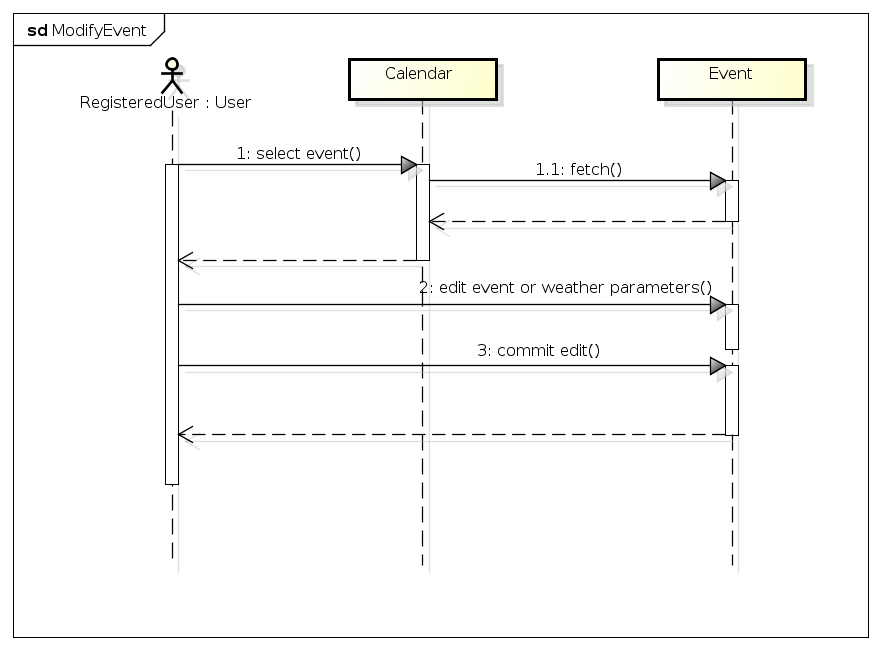
\includegraphics[width=1\textwidth]{../UMLDiagram/sequence/ModifyEvent/ModifyEvent.png}
    \caption{Sequence Diagram of event's modification}
     \label{fig:modseqdiag}
     \end{figure}
   \end{center}  
\subsubsection{Event deletion}
\begin{center}
 \begin{figure}[H]
    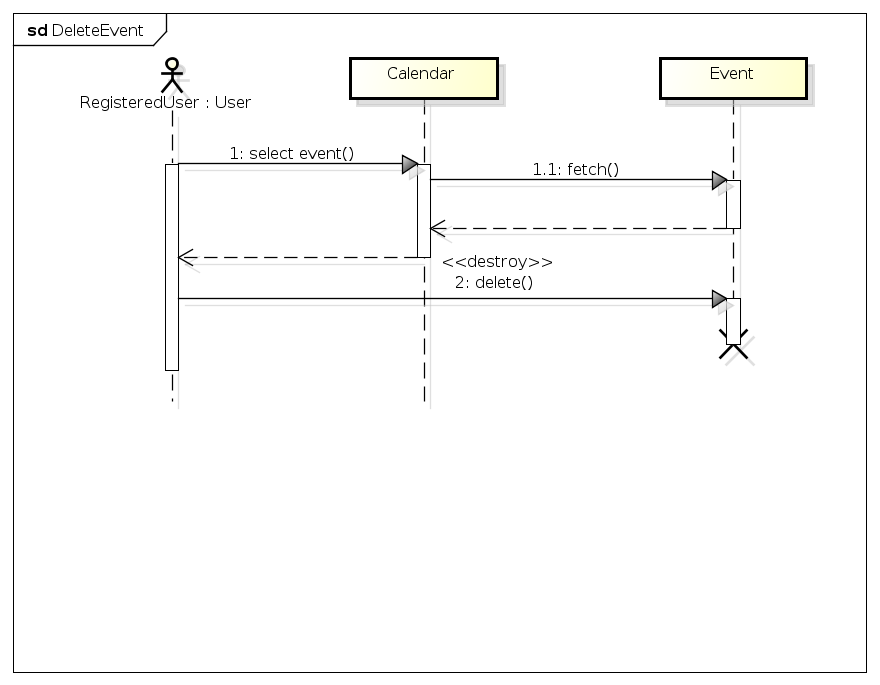
\includegraphics[width=1\textwidth]{../UMLDiagram/sequence/DeleteEvent/DeleteEvent.png}
    \caption{Sequence Diagram of event's deletion}
     \label{fig:delseqdiag}
     \end{figure}
   \end{center}  
\subsubsection{Invitation}
\begin{center}
 \begin{figure}[H]
    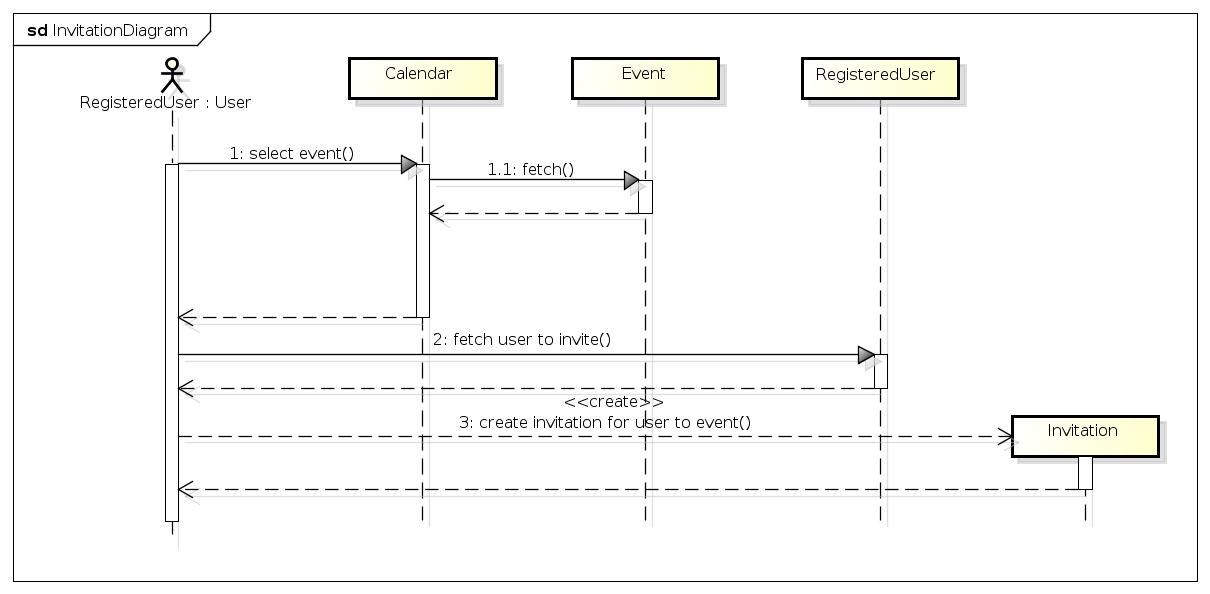
\includegraphics[width=1\textwidth]{../UMLDiagram/sequence/InvitationDiagram/InvitationDiagram.png}
    \caption{Sequence Diagram of an invitation}
     \label{fig:invitseqdiag}
     \end{figure}
   \end{center}  
\subsubsection{Invite notification}
\begin{center}
 \begin{figure}[H]
    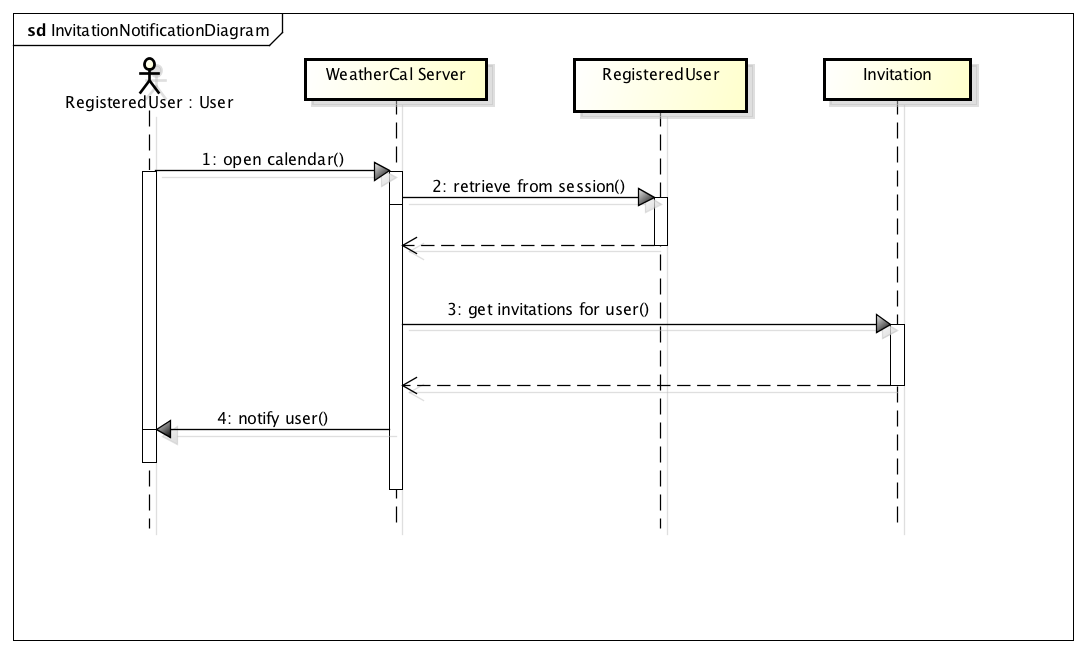
\includegraphics[width=1\textwidth]{../UMLDiagram/sequence/InvitationNotificationDiagram/InvitationNotificationDiagram.png}
    \caption{Sequence Diagram of an invitation's notification}
     \label{fig:notseqdiagr}
     \end{figure}
   \end{center}  
\subsubsection{Modify participation}
\begin{center}
 \begin{figure}[H]
    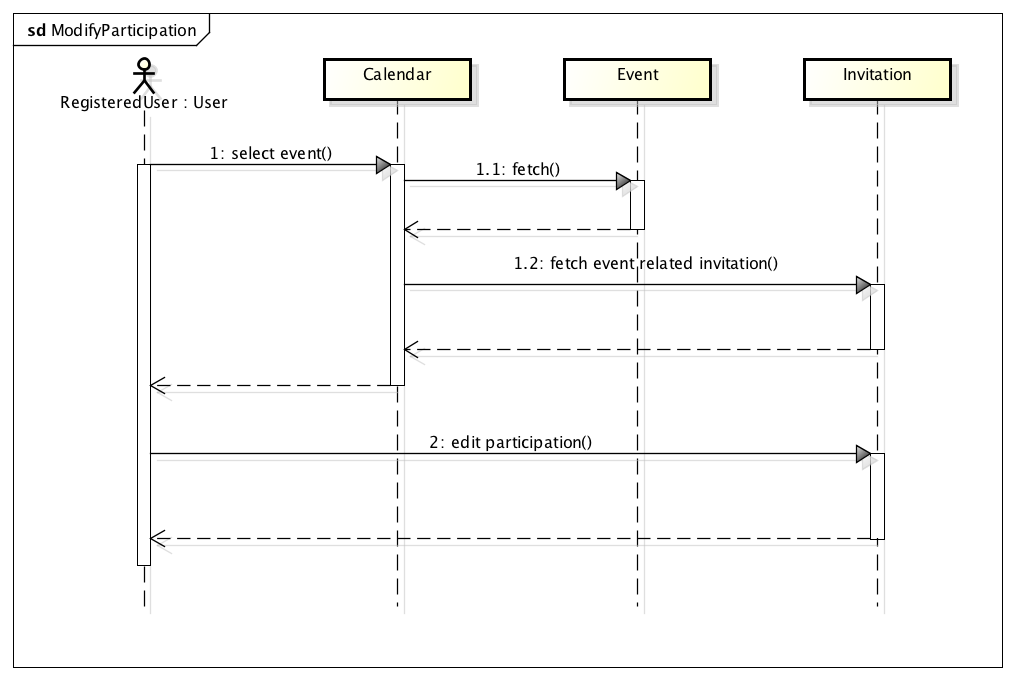
\includegraphics[width=1\textwidth]{../UMLDiagram/sequence/ModifyParticipation/ModifyParticipation.png}
    \caption{Modify participation Sequence Diagram}
     \label{fig:modpartseqdiag}
     \end{figure}
   \end{center}  
\section{Alloy}







